\documentclass[11pt,a4paper]{article}

\usepackage[utf8]{inputenc}
\usepackage[T1]{fontenc}
\usepackage[spanish,es-nodecimaldot]{babel}
\usepackage{lmodern}
\usepackage{geometry}
\usepackage{graphicx}
\usepackage{booktabs}
\usepackage{float}
\usepackage{amsmath}
\usepackage{xcolor}
\usepackage[hidelinks]{hyperref}

\geometry{margin=2.5cm}
\graphicspath{{../informe/figuras/}}

\title{Informe técnico\\La falla del nodo 214}
\author{Análisis del dataset de Energía y datos geo-agrónomos}
\date{\today}

\begin{document}

\maketitle

\begin{abstract}
Este informe analiza técnicamente el problema de negocio ``La Falla del Nodo 214'' mediante tres enfoques complementarios: causalidad temporal entre factor de potencia y voltaje, priorización geo-agrónoma de sensores para infraestructura hídrica y modelación predictiva de la demanda mediante ARIMAX. Los resultados se interpretan con un nivel de significancia de $\alpha=0.05$ y se apoyan en las figuras generadas desde el notebook \texttt{taller\_practico\_03.ipynb}.
\end{abstract}

\section{Contexto y alcance}

El problema plantea que, cuando el Precio Spot (\texttt{Ener\_2}) supera un umbral crítico, el flujo hacia ciertos nodos destino puede interrumpirse y coincidir con una anomalía térmica georreferenciada. El objetivo de este documento es responder las preguntas P1--P3 con evidencia estadística y gráfica. La interpretación causal se entiende en el sentido de precedencia temporal de Granger; no equivale, por sí sola, a una prueba de causalidad física.

\section{P1. Causalidad y redes}

\subsection{Método}

Se aplicó la prueba de causalidad de Granger entre \texttt{Ener\_10} (factor de potencia, denominado Potencia en las figuras) y \texttt{Ener\_9} (voltaje), evaluando rezagos de 1 a 10. Para cada dirección se reportó el menor valor-$p$. Además, se construyó un grafo dirigido a partir de las relaciones \texttt{Source\_Node}--\texttt{Target\_Node} y se calcularon la centralidad de intermediación (Betweenness Centrality) y la centralidad de grado.

\begin{figure}[H]
    \centering
    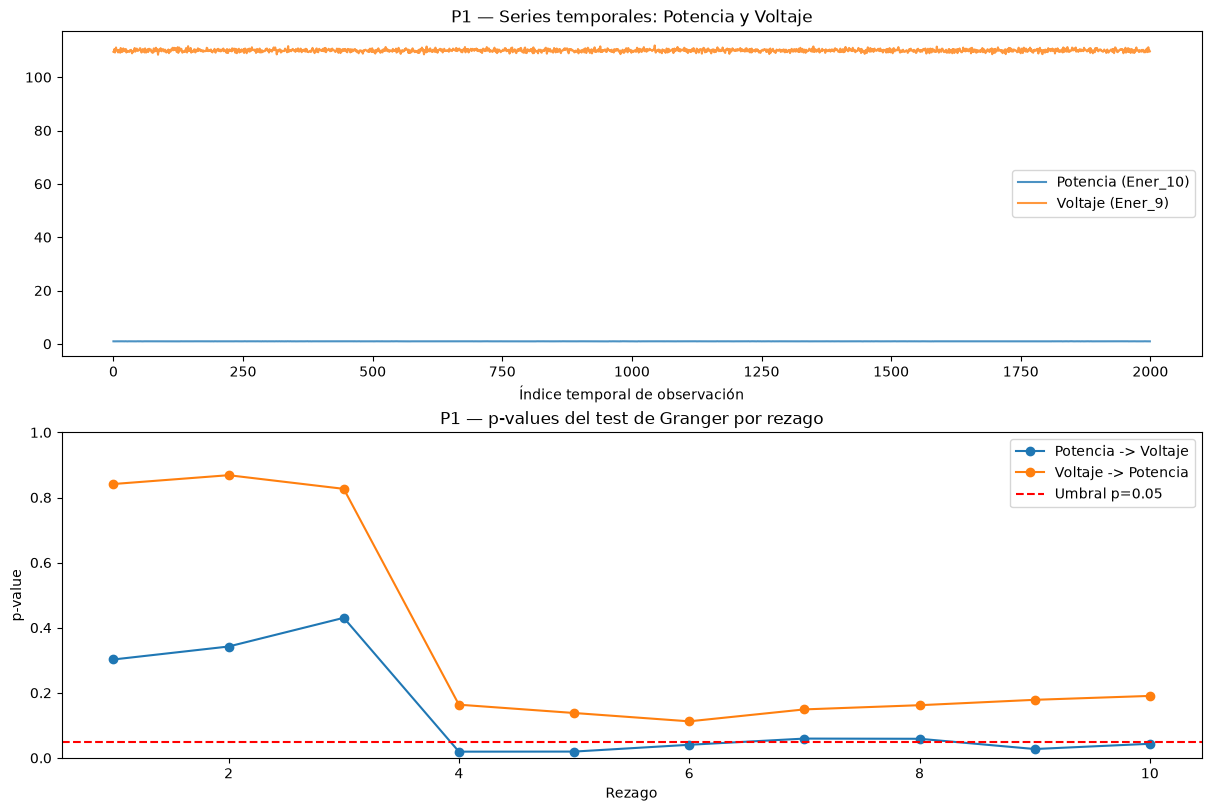
\includegraphics[width=0.98\textwidth]{p1.png}
    \caption{Series de Potencia y Voltaje, junto con los valores-$p$ de la prueba de Granger por rezago.}
    \label{fig:p1}
\end{figure}

\subsection{Resultados}

La dirección \texttt{Ener\_10 $\rightarrow$ Ener\_9} presentó evidencia de precedencia temporal: el menor valor-$p$ fue $0.0193$ en el rezago 4, por debajo de $0.05$. En la dirección inversa \texttt{Ener\_9 $\rightarrow$ Ener\_10}, el menor valor-$p$ fue $0.1125$ en el rezago 6, por lo que no se rechazó la hipótesis nula al nivel de significancia adoptado.

El grafo energético contiene 70 nodos y 865 aristas. En la representación observada, la Betweenness Centrality resultó cero para todos los nodos, incluido el nodo 214. Esto es consistente con una topología esencialmente de conexiones directas origen--destino, sin rutas geodésicas alternativas que atraviesen nodos intermedios. Para complementar esta limitación estructural, se consultó la centralidad de grado: el nodo 214 obtuvo un valor de $0.2319$, lo que lo sitúa como un nodo con alta conectividad relativa.

\subsection{Respuesta de negocio}

La evidencia estadística sugiere que cambios en el factor de potencia anticipan cambios posteriores en el voltaje. Por tanto, una falla en un nodo muy conectado como el 214 puede producir una perturbación amplia: pérdida de flujo en múltiples enlaces, redistribución de carga, desviaciones de voltaje y mayor probabilidad de inestabilidad en nodos vecinos. Sin embargo, no debe afirmarse que el nodo 214 sea el de mayor Betweenness con este grafo concreto, porque todos los valores de Betweenness son cero. La recomendación operativa es fortalecer el monitoreo de voltaje y potencia alrededor de sus enlaces, definir rutas de contingencia y recalcular la centralidad sobre un grafo agregado por intervalos o con enlaces de transmisión completos si se desea identificar intermediación real.

\section{P2. Optimización geo-agrónoma}

\subsection{Método}

Las coordenadas GPS se suavizaron mediante una mediana móvil de ventana 5 para reducir ruido espacial. Se definió como zona prioritaria la intersección de dos condiciones: NDVI menor o igual al percentil 25 y varianza del viento \texttt{Agro\_10} mayor o igual al percentil 75. Estos umbrales identifican simultáneamente estrés vegetativo y exposición eólica elevada.

\begin{figure}[H]
    \centering
    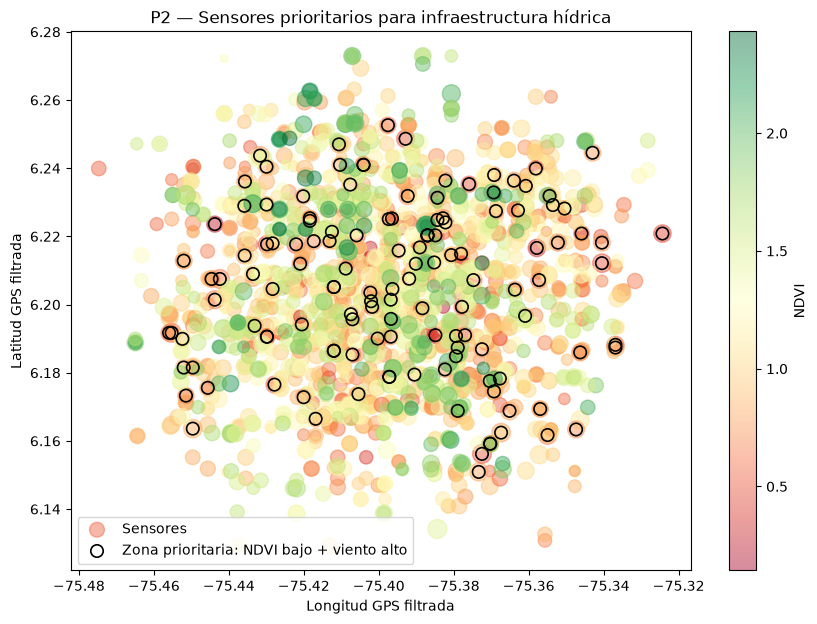
\includegraphics[width=0.86\textwidth]{p2.png}
    \caption{Distribución espacial de sensores; el contorno negro identifica la combinación de NDVI bajo y varianza del viento alta.}
    \label{fig:p2}
\end{figure}

\subsection{Resultados y recomendación}

Los umbrales calculados fueron NDVI $\leq 0.8619$ y varianza del viento $\geq 6.0998$. La intersección identificó 132 sensores de 2\,000, equivalente al 6.6\% de las observaciones. La concentración de estos sensores representa una señal de vulnerabilidad agronómica: menor vigor vegetal en una zona donde el viento puede aumentar la evapotranspiración, la deriva del riego y la heterogeneidad de aplicación.

Se recomienda priorizar inversión hídrica focalizada en las zonas delimitadas, comenzando por infraestructura de riego presurizado y sectorizado, almacenamiento o regulación local y sensores de humedad de suelo. El diseño debería incorporar protección contra viento --por ejemplo, cortinas rompevientos donde sea agronómicamente viable-- y control de caudal por sector. La inversión no debe distribuirse uniformemente sobre toda el área: el 6.6\% priorizado permite iniciar un piloto, medir reducción del estrés y escalar solo si mejora el uso de agua y el NDVI. La priorización es asociativa; para dimensionar tuberías y reservorios se requiere validar pendiente, textura de suelo, disponibilidad hídrica y caudal de diseño.

\section{P3. Analítica predictiva}

\subsection{Método}

Se ajustaron dos modelos SARIMAX para la demanda \texttt{Ener\_1}. El modelo base incorporó Temperatura como variable exógena; el segundo agregó la importancia del nodo de origen, representada por su centralidad. Se compararon modelos con la misma muestra y se seleccionó el orden ARIMA mediante el procedimiento utilizado en el notebook.

\begin{figure}[H]
    \centering
    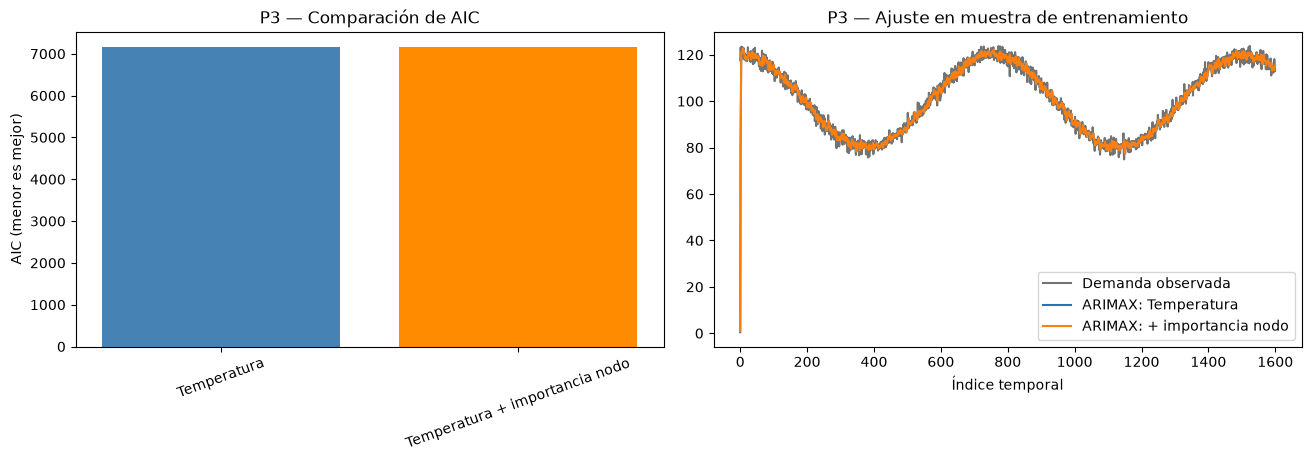
\includegraphics[width=0.99\textwidth]{p3.png}
    \caption{Comparación del AIC y ajuste en la muestra de entrenamiento para los dos modelos ARIMAX.}
    \label{fig:p3}
\end{figure}

\subsection{Resultados}

\begin{table}[H]
    \centering
    \caption{Comparación de especificaciones ARIMAX.}
    \label{tab:aic}
    \begin{tabular}{lccc}
        \toprule
        Modelo & Orden ARIMA & AIC & $\Delta$AIC frente al base \\
        \midrule
        Temperatura & (2,1,0) & 7167.695 & 0.000 \\
        Temperatura + importancia del nodo & (2,1,0) & 7169.439 & +1.744 \\
        \bottomrule
    \end{tabular}
\end{table}

El AIC no mejora al incluir la importancia del nodo: aumenta en 1.744 unidades. Dado que un AIC menor es preferible, la variable de centralidad no aporta capacidad explicativa suficiente para justificar su inclusión en esta especificación. La conclusión es específica del conjunto de datos, del periodo analizado y de la forma en que se construyó la centralidad; no implica que la topología sea irrelevante en todos los horizontes o regímenes operativos.

\section{Preguntas de Verificacion}

\begin{enumerate}
    \item \textbf{Sobre la Estacionariedad: ¿Por qué no es válido aplicar un análisis de correlación de Pearson directamente sobre una serie con tendencia (como el NDVI o el Precio de Exportación)?}


    El coeficiente de Pearson mide covarianza lineal entre dos variables, y su interpretación válida exige que ambas series tengan media y varianza constantes en el tiempo. Cuando una serie tiene tendencia, como el NDVI, Pearson arrojará una correlación alta aunque no exista relación causal ni estructural entre ellas. Tambien, la fórmula de Pearson asume que la dispersión alrededor de la media es estable, con tendencia, la media cambia en cada punto, por lo que el estadístico pierde su interpretación probabilística
    

    \item \textbf{Sobre el SNR: ¿Qué impacto tuvo el ruido de 5dB en la estimación de los coeficientes del modelo ARMA comparado con la versión Clean?}


    Un SNR de 5dB es relativamente bajo, por lo que el impacto sobre la estimación ARMA suele incluir sesgo en los coeficientes, especialmente en la parte MA: el ruido blanco añadido se confunde con la estructura de media móvil del modelo, deformando las estimaciones de los parámetros MA más que las AR. Ademas, con menor SNR, los intervalos de confianza de los coeficientes se ensanchan, el modelo clean da estimaciones más precisas y estables frente a distintas semillas.


    \item \textbf{Sobre la Topología: ¿Cómo cambia la interpretación de un fallo en un sensor si este es un "Bridge"(puente) en el grafo de la red?}


    En teoría de grafos, un puente es una arista cuya eliminación desconecta el grafo en dos o más componentes. Que un sensor sea un bridge cambia la interpretación de su fallo. Si falla un sensor no bridge, la red se reconfigura y las rutas alternativas mantienen la conectividad. Si falla un bridge, una parte completa de la red queda incomunicada, sin ninguna ruta alternativa.
    

    \item  Sobre la Geo-Inteligencia: ¿Cómo influye la posición geográfica en la varianza de la señal capturada?

    La posición geográfica afecta la varianza capturada por un sensor ya que sensores próximos entre sí tienden a mostrar menor varianza relativa entre ellos, mientras que sensores dispersos captan mayor heterogeneidad ambiental.


\end{enumerate}


\section{Conclusiones técnicas}

\begin{enumerate}
    \item Existe evidencia de precedencia temporal de Potencia sobre Voltaje, pero no en la dirección inversa. Un nodo con alta conectividad puede propagar una falla aunque su Betweenness sea nula en la topología actual.
    \item La zona prioritaria de infraestructura hídrica combina NDVI bajo y viento alto. Se identificó el 6.6\% de los sensores como primera área de intervención, sujeto a validación agronómica y de ingeniería.
    \item La centralidad del nodo de origen no mejora el ARIMAX de demanda bajo el criterio AIC. El modelo con Temperatura permanece como la alternativa preferible entre las dos comparadas.
\end{enumerate}

\end{document}
